% 原书 p.287–p.298（PDF p.295–p.306）
\section{层速成（A Crash Course on Sheaf）}

% >>> p295
本节中，我们快速回顾层论的一些背景，其中包含后文发展所需的全部要素。更多细节见
[33] 第 1 节、[112] 第 II 章第 1 节以及 [135] 第 II 章。先固定一些记号。固定基域
$\mathbf{k}$，记 $\operatorname{Mod}(\mathbf{k})$ 为 $\mathbf{k}$-模范畴。对拓扑空间
$X$，$X$ 的一切开子集之集记作 $\operatorname{Op}(X)$。注意 $\operatorname{Op}(X)$ 也可以看作一个范畴，其对象集
为 $\operatorname{Ob}(\operatorname{Op}(X))=\{U\subset X\mid U\ \text{是开的}\}$，而 hom-集由
下式定义：
\[
  \hom_{\operatorname{Op}(X)}(U,V)\,\bigl(=\operatorname{Mor}_{\operatorname{Op}(X)}(U,V)\bigr)
  =\begin{cases}
    * & \text{若 } U\subset V,\\
    \varnothing & \text{否则}
  \end{cases}
\]

\begin{keytakeaways}
\begin{itemize}
  \item 几何图像：层是「把局部数据粘成整体数据」的装置——预层给出开集到模的函子，
        层再加上唯一性与粘合两条公理；茎则记录一点处的无穷小局部信息。
  \item 数学工具：预层／层（定义 10.2.1、10.2.2）、态射与层化（练习 10.2.1）、
        有向集与有向极限（定义 10.2.3--10.2.5）、茎（定义 10.2.6）、
        拉回 $f^{-1}$ 与前推 $f_*$（定义 10.2.7、10.2.8）。
  \item 关键结论：$\gamma$-拓扑下的层与持续模等价（例 10.2.4 (iii)）；可构造层分解为
        区间常值层之直和（定理 10.2.1），这正是定理 5.2.1 的层类比。
  \item 与辛几何的联系：层的 $\Z$-裁剪（式 (10.10)）与六种运算（定义 10.2.7 起）
        是后文把辛对象「代数化」的基本操作。
\end{itemize}
\end{keytakeaways}

\begin{wdefn}{10.2.1}
  设 $X$ 是拓扑空间。$\mathbf{k}$-模的\textbf{预层}（presheaf）是一个反变函子
  $\mathcal{F}\colon\operatorname{Op}(X)\to\operatorname{Mod}(\mathbf{k})$。具体地说，对任意
  $U\in\operatorname{Op}(X)$，$\mathcal{F}(U)$ 是一个 $\mathbf{k}$-模；并且对任意 $U\subset V$，
  存在一个称为\textbf{限制映射}的映射，记作
  $\operatorname{res}_{V,U}\colon\mathcal{F}(V)\to\mathcal{F}(U)$，使得
  $\operatorname{res}_{U,U}=\mathbf{1}_{\mathcal{F}(U)}$；且对任意
  $U\subset V\subset W$，有
  $\operatorname{res}_{V,U}\circ\operatorname{res}_{W,V}
  =\operatorname{res}_{W,U}$。此外，$\mathcal{F}(U)$ 中的任何元素称为 $U$ 上的
  \textbf{截面}（section），通常记作 $s\in\mathcal{F}(U)$。
\end{wdefn}

% >>> p296
\begin{wrem}{10.2.1}
  用同样的方式可以定义阿贝尔群的预层：只需把目标范畴由
  $\operatorname{Mod}(\mathbf{k})$ 换成阿贝尔群范畴。
\end{wrem}

\begin{wdefn}{10.2.2}
  $\mathbf{k}$-模的\textbf{层}（sheaf）是一个 $\mathbf{k}$-模预层，且满足下述条件：
  \begin{enumerate}[label=(\roman*)]
    \item （唯一性）设 $U=\bigcup_{i\in I}U_i$ 是带覆盖 $\{U_i\}_{i\in I}$ 的开集，
          且对任意截面 $s,t\in\mathcal{F}(U)$，若对任意 $i\in I$ 有
          $\operatorname{res}_{U,U_i}(s)=\operatorname{res}_{U,U_i}(t)$，则
          $s=t$。
    \item （粘合）设 $U=\bigcup_{i\in I}U_i$ 是带覆盖 $\{U_i\}_{i\in I}$ 的开集。
          给定一族的截面 $\{s_i\in\mathcal{F}(U_i)\}_{i\in I}$，满足对一切
          $i,j\in I$ 有
          $\operatorname{res}_{U_i,U_i\cap U_j}(s_i)
          =\operatorname{res}_{U_j,U_i\cap U_j}(s_j)$，则存在截面
          $s\in\mathcal{F}(U)$，使得
          $\operatorname{res}_{U,U_i}(s)=s_i$。
  \end{enumerate}
\end{wdefn}

\begin{wrem}{10.2.2}
  定义 10.2.2 中的条件 (i) 等价于下述条件：若对任意 $i\in I$ 有
  $\operatorname{res}_{U,U_i}(s)=0$，则 $s=0$。
\end{wrem}

层之间的态射 $\varphi$（实际上是其底层预层之间的态射）应当定义为两个函子之间的自然
变换（见定义 10.2.1）——这是用范畴论语言的说法。换言之，$\varphi$ 需要与限制映射
相容。具体地说，给定两个层 $\mathcal{F}$ 与 $\mathcal{G}$，态射
$\varphi\colon\mathcal{F}\to\mathcal{G}$ 是一族 $\mathbf{k}$-线性映射
$\{\varphi(U)\}_{U\in\operatorname{Op}(X)}$，使得下图交换。

\begin{figure}[htbp]
  \centering
  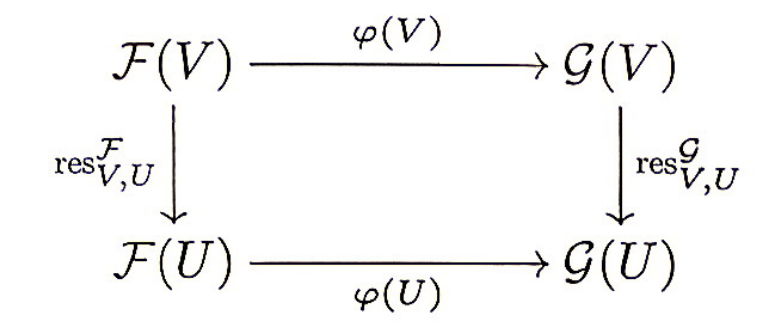
\includegraphics[width=0.55\linewidth]{figures/fig_p296_1.png}
  \caption*{层之间态射的交换图（原书 p.288 示意图，无编号；PDF p.296）}
\end{figure}

此外，若对任意 $U\in\operatorname{Op}(X)$ 都有 $\varphi(U)$ 是同构，则称 $\varphi$ 是同构。

下述练习表明，任何预层 $\mathcal{F}$ 都可以被修改为一个层，记作
$\mathcal{F}^+$。特别地，若 $\mathcal{F}$ 本身已是层，则
$\mathcal{F}\simeq\mathcal{F}^+$，其中同构如上定义（见练习中的 (ii)）。注意这个练习
依赖于\textbf{茎}（stalk）这一概念——层 $\mathcal{F}$ 在一点处的茎记作
$\mathcal{F}_x$（它最终建立在正向极限的概念之上），故读者可以先跳到定义 10.2.6 或
定义 10.2.5 再回来做这个练习。

\begin{wexer}{10.2.1}
  设 $X$ 是拓扑空间，$\mathcal{F}$ 是 $X$ 上 $\mathbf{k}$-模的预层。按下述方式定义
  一个对应 $\mathcal{F}^+\colon\operatorname{Op}(X)\to\operatorname{Mod}(\mathbf{k})$：
  $\mathcal{F}^+(U)$ 由一切映射 $s\colon U\to\bigsqcup_{x\in U}\mathcal{F}_x$
  组成，使得对 $x\in U$ 有 $s(x)\in\mathcal{F}_x$，并且存在 $x$ 的一个开邻域
  $V\subset U$ 与截面 $t\in\mathcal{F}(V)$，使得对一切 $y\in V$ 有
  $t_y=s(y)$。
  \begin{enumerate}[label=(\roman*)]
    \item 证明 $\mathcal{F}^+$ 是 $\mathbf{k}$-模的层，称为 $\mathcal{F}$ 的
          \textbf{层化}（sheafification）。
    \item 证明：若 $\mathcal{F}$ 是层，则 $\mathcal{F}$ 与 $\mathcal{F}^+$
          之间存在同构。
    \item 注意存在一个自然映射 $i\colon\mathcal{F}\to\mathcal{F}^+$，定义如下：
          对任意 $U\in\operatorname{Op}(X)$ 与截面 $s\in\mathcal{F}(U)$，令
          \[
            i(U)(s):=\bigsqcup_{x\in U}s_x\in\mathcal{F}^+(U).
          \]
          证明：给定任意预层态射 $\varphi\colon\mathcal{F}\to\mathcal{G}$，其中
          $\mathcal{G}$ 是层，则存在唯一的层态射
          $\varphi^+\colon\mathcal{F}^+\to\mathcal{G}$，使得
          $\varphi^+\circ i=\varphi$。
    \item 在光滑流形 $M$ 上，考虑开子集 $U\subset M$ 上的恰当形式预层
          $\Omega^p_{\mathrm{exact}}$，其定义为
          $\Omega^p_{\mathrm{exact}}(U)=\{\Omega^p(U)\ \text{中的恰当 } p\ \text{-形式}\}$。
          计算其层化 $(\Omega^p_{\mathrm{exact}})^+$。
  \end{enumerate}
\end{wexer}

% >>> p297
\begin{wexer}{10.2.2}
  设 $\varphi\colon\mathcal{F}\to\mathcal{G}$ 是层态射。证明：由
  \[
    \ker(\varphi)(U):=\ker\bigl(\varphi(U)\bigr)
  \]
  对任意 $U\in\operatorname{Op}(X)$ 定义的 $\ker(\varphi)$ 也是层。不过要注意，
  $\operatorname{im}(\varphi)$ 并不总是层（见例 10.2.7）。为得到层，需要考虑
  $\operatorname{im}(\varphi)$ 的层化，仍记作 $\operatorname{im}(\varphi)$。
\end{wexer}

\begin{wexam}{10.2.1}
  设 $X$ 是拓扑空间。\textbf{常值层}（constant sheaf，秩为 $N$ 的
  $\mathbf{k}$-模），记作 $\mathbf{k}_X$，是下述预层的层化：对任意非空
  $U\in\operatorname{Op}(X)$，定义
  \[
    \mathbf{k}_X(U)=\mathbf{k}^N
  \]
  对某个固定的整数 $N>0$，它与 $U\in\operatorname{Op}(X)$ 无关。当 $U=\varnothing$ 时，令
  $\mathbf{k}_X(U)=\mathbf{k}_X(\varnothing)=0$。此时对任意非空开集
  $U,V\in\operatorname{Op}(X)$，限制映射
  $\operatorname{res}_{U,V}=\mathbf{1}_{\mathbf{k}^N}$。注意：为使记号
  $\mathbf{k}_X$ 简洁，我们\emph{不}把秩的信息（例如 $N$）写进 $\mathbf{k}_X$
  这一记号中。
  \hfill$//$
\end{wexam}

% [Tutor Note: 易错预警——常值层不等于「常值预层」$U\mapsto\mathbf{k}^N$：后者不满足
% 粘合公理，例如 $X$ 不连通时，在无交并的两个开集上分别取常值 $1$ 的截面可以粘成
% 局部常值而非整体的常值截面。层化后的 $\mathbf{k}_X$ 在连通开集上取 $\mathbf{k}^N$，
% 在一般开集上取的是「局部常值函数」构成的 $\mathbf{k}^N$-模。这一区别在
% 例 10.2.11 中会被用来计算裁剪层在开区间上的截面。]

层的\emph{局部信息}可以由其\textbf{茎}来捕捉。为说明这一点，需要\textbf{正向极限}
（direct limit）这一记号。正向极限是 6.3 节 (6.16) 中引入的逆向极限的「对偶」——
更严格地说，是它的伴随算子。我们先从\textbf{有向集}与\textbf{有向系统}的定义开始。

\begin{wdefn}{10.2.3}
  \textbf{有向集}（directed set）$(I,\preceq)$ 是一个偏序集，使得对任意
  $i,j\in I$，存在 $k\in I$ 使 $i\preceq k$ 且 $j\preceq k$。
\end{wdefn}

\begin{wexam}{10.2.2}
  任何全序集都是有向集，因为我们总可以取所需的 $k$ 为 $\max\{i,j\}$。
  \hfill$//$
\end{wexam}

下面给出有向集的更多例子。

\begin{wexam}{10.2.3}
  (i) 取 $(I,\preceq)$ 为整数 $(\Z,\le)$ 配以通常的（全）序。(ii) 给定拓扑空间
  $X$ 与点 $x\in X$，考虑集合
  \[
    \operatorname{Op}(X,x):=\{U\in\operatorname{Op}(X)\mid x\in U\}.
  \]

% >>> p298
  于是可以取 $(I,\preceq)=(\operatorname{Op}(X,x),\supseteq)$，其中（偏）序由包含关系
  $\supseteq$ 给出。

  (iii) 取 $(I,\preceq)=(\R,\le)$，即全体实数之集，它按 $\R$ 中的标准序全序化。本质
上以同样的方式，我们可以考虑 $\R$ 上的 $\gamma$-\textbf{拓扑}（$\gamma$-topology），
它指的是：其开子集由 $\R$ 中形如 $(a,\infty)$（$a\in\R$）的开子集组成。在这个拓扑
下，$\R$ 记作 $\R_\gamma$。取 $(I,\preceq)$ 为 $(\operatorname{Op}(\R_\gamma),\supseteq)$，其中
$\supseteq$ 是包含关系。注意这个包含关系在 $\operatorname{Op}(\R_\gamma)$ 上给出一个全序。此外，
存在从 $(\R,\le)$ 到 $(\operatorname{Op}(\R_\gamma),\supseteq)$ 的保序同构，简单地由
$a\mapsto(a,\infty)$ 给出。这样，我们有
\[
  a\le b\quad\Longrightarrow\quad(a,\infty)\supseteq(b,\infty).
\]
  因此，作为有向系统，可以放心地把 $(\R,\le)$ 与 $(\operatorname{Op}(\R_\gamma),\supseteq)$
  等同起来。
  \hfill$//$
\end{wexam}

\begin{wrem}{10.2.3}
  有向集可以看作一个范畴：对象
  $\operatorname{Ob}=\{i\in I\}$，态射为：若 $i\preceq j$ 则
  $\operatorname{Mor}(i,j)=\{*\}$，否则 $\operatorname{Mor}(i,j)=\varnothing$。
\end{wrem}

\begin{wdefn}{10.2.4}
  $\mathbf{k}$-模的\textbf{有向系统}（directed system，定义在有向集 $(I,\preceq)$
  上）是一个共变函子 $\varphi\colon(I,\preceq)\to\operatorname{Mod}(\mathbf{k})$。
  具体地说，对任意 $i\in I$，像 $\varphi(i)$ 是一个 $\mathbf{k}$-模；并且对任意
  $i\preceq j$，存在一个 $\mathbf{k}$-线性映射，记作 $\varphi_{ij}$，从
  $\varphi(i)$ 到 $\varphi(j)$，满足 $\varphi_{ii}=\mathbf{1}_{\varphi(i)}$，且
  当 $i\preceq j\preceq k$ 时 $\varphi_{ik}=\varphi_{jk}\circ\varphi_{ij}$。
\end{wdefn}

用同样的方式，可以定义阿贝尔群的有向系统，或任何其他代数或拓扑对象的有向系统。

承接例 10.2.3，下面是一些有向系统的例子。

\begin{wexam}{10.2.4}
  (i) 给定一列开子集 $\{U_i\}_{i\in\Z}$，使得对任意 $i\in\Z$ 有
  $U_i\subset U_{i+1}$。则可以定义函子
  $\varphi\colon(\Z,\le)\to(\{U_i\}_{i\in\Z},\subseteq)$ 为
  \[
    \varphi(i)=U_i\quad\text{且}\quad
    \varphi_{ij}=\text{包含映射 } U_i\hookrightarrow U_j
  \]
  （当 $i\le j$ 时）。这个 $\varphi$ 定义了有向系统。

  (ii) 给定拓扑空间 $X$ 上的层 $\mathcal{F}$，对固定的 $x\in X$，考虑限制
  $\mathcal{F}|_{\operatorname{Op}(X,x)}$。则
  \[
    \mathcal{F}|_{\operatorname{Op}(X,x)}\colon(\operatorname{Op}(X,x),\supseteq)
    \to\operatorname{Mod}(\mathbf{k})
  \]
  是有向系统。

  (iii) 考虑 $\R_\gamma$ 上（配以 $\gamma$-拓扑，见例 10.2.3 的 (iii)）的
  $\mathbf{k}$-模层。具体地说，我们有一个映射
  $\mathcal{F}\colon(\operatorname{Op}(\R_\gamma),\supseteq)\to\operatorname{Mod}(\mathbf{k})$，
  其中限制映射
  $\operatorname{res}_{(a,\infty),(b,\infty)}\colon
  \mathcal{F}((a,\infty))\to\mathcal{F}((b,\infty))$ 由序 $a\le b$ 诱导。这个层
  自身给出一个有向系统。这样的层有时也称为\textbf{持续 $\mathbf{k}$-模}
  （persistence $\mathbf{k}$-module，cf.\ 定义 5.2.1）。
  \hfill$//$
\end{wexam}

% [Tutor Note: 含糊点拨——例 10.2.4 (iii) 是本章与第 5 章的接口：$\R_\gamma$ 上的层
% 与「以 $\R$ 为参数的持续 $\mathbf{k}$-模」是同一件事（对象与态射一一对应）。这正是
% 定理 10.2.1 能与定理 5.2.1（持续模的区间分解）平行陈述的原因：层论把条形码的语言
% 推广到更一般的空间，而 $\R_\gamma$ 上的可构造层分解为区间常值层之直和，恰好就是
% 条形码。阅读时建议把 $V_t=\mathrm{SH}^{(\cdot)}$ 的过滤族直接理解为
% $\operatorname{Op}(\R_\gamma)$ 上的一个层。]

最后，我们可以给出正向极限的定义。

% >>> p299
\begin{wdefn}{10.2.5}
  给定有向系统 $\varphi\colon(I,\preceq)\to\operatorname{Mod}(\mathbf{k})$，其
  \textbf{正向极限}（directed limit）定义为
  \[
    \varinjlim_{i\in I}\varphi(i):=\left.
    \bigsqcup_{i\in I}\varphi(i)\right/\sim,
  \]
  其中 $x_i\in\varphi(i)$ 与 $x_j\in\varphi(j)$ 等价（就记号 $\sim$ 而言）当且仅当
  存在 $k\in I$ 与 $i\preceq k$、$j\preceq k$，使得在 $\varphi(k)$ 中有
  $\varphi_{ik}(x_i)=\varphi_{jk}(x_j)$。
\end{wdefn}

由定义 10.2.5 立即得到下述观察。

\begin{enumerate}[label=(\roman*)]
  \item 存在自然映射 $\pi_i\colon\varphi(i)\to\varinjlim_{i\in I}\varphi(i)$，
        它把 $\varphi(i)$ 中元素映到其等价类。此外，按定义，这些自然投影满足下述
        关系：对 $i\preceq j$，有 $\pi_j\circ\varphi_{ij}=\pi_i$。
  \item 若存在 $i_0\in I$，使得对任意 $i_0\preceq i$、$i_0\preceq j$ 都有
        $\varphi_{ij}$ 是同构，则存在 $k\in I$ 与 $i_0\preceq k$，使得
        $\varinjlim_{i\in I}\varphi(i)=\varphi(k)$。
  \item 比 (ii) 更一般地，若在 $(I,\preceq)$ 中存在一个\textbf{穷竭}（exhausting）
        （子）序列 $(J,\preceq)$（其意义是：对任意 $i\in I$，总存在 $j\in J$
        使 $i\preceq j$），使得对任意 $j_1\preceq j_2\in J$，映射
        $\varphi_{j_1j_2}$ 都是同构，则
        \[
          \varinjlim_{i\in I}\varphi(i)=\varphi(j_\ast)
        \]
        对某个充分大的 $j_\ast\in J$ 成立。这提供了通过寻找穷竭（子）序列
        $(J,\preceq)$ 来计算正向极限的有效方法（cf.\ 事实 6.3.1）。
\end{enumerate}

\begin{wexer}{10.2.3}
  设 $\varphi\colon(I,\preceq)\to\operatorname{Mod}(\mathbf{k})$ 是有向系统。证明：
  其正向极限可以等价地定义为一个元素 $X$ 连同一族 $\mathbf{k}$-线性映射
  $\pi_i\colon\varphi(i)\to X$（$i\in I$），满足对任意 $i\preceq j$ 有
  $\pi_j\circ\varphi_{ij}=\pi_i$，并且使得：对任意 $Y$ 与态射
  $f_i\colon\varphi(i)\to Y$（满足对任意 $i\preceq j$ 有
  $f_j\circ\varphi_{ij}=f_i$），存在唯一的映射 $u\colon X\to Y$，使下图交换。

  \begin{figure}[htbp]
    \centering
    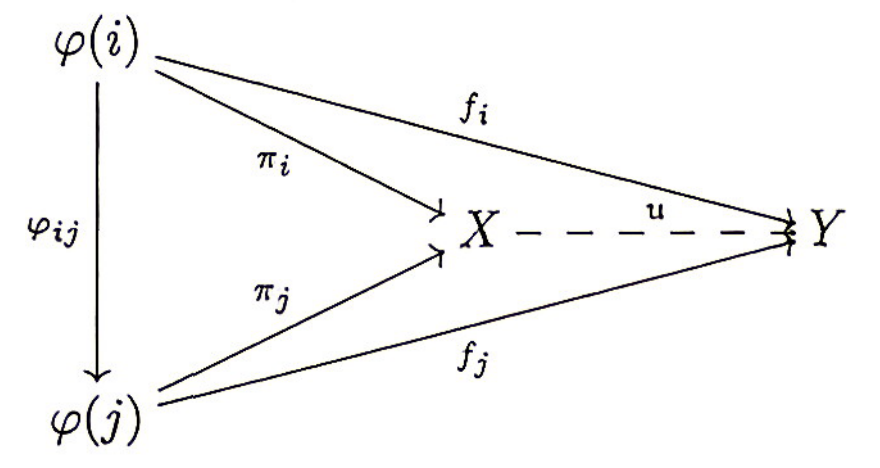
\includegraphics[width=0.52\linewidth]{figures/fig_p299_1.png}
    \caption*{练习 10.2.3 中正向极限的泛性质（原书 p.291 示意图，无编号；PDF p.299）}
  \end{figure}

  作为直接推论，证明对例 10.2.4 中的有向系统 (i)，有
  $\varinjlim_{i\in I}\varphi(i)=\varinjlim_{i\in I}U_i=\bigcup_{i\in I}U_i$。
\end{wexer}

基于正向极限的定义，现在可以定义层的茎。

\begin{wdefn}{10.2.6}
  给定拓扑空间 $X$ 上 $\mathbf{k}$-模的层 $\mathcal{F}$，对任意固定的
  $x\in X$，定义 $\mathcal{F}$ 在 $x\in X$ 处的\textbf{茎}（stalk）为
  \[
    \mathcal{F}_x:=\varinjlim_{U\in\operatorname{Op}(X,x)}\mathcal{F}(U).
  \]
\end{wdefn}

% [Tutor Note: 易错预警——「茎」与「纤维」不是一回事。茎
% $\mathcal{F}_x=\varinjlim_{U\ni x}\mathcal{F}(U)$ 是 $x$ 的一个\emph{邻域基}上的
% 正向极限，其元素是截面的「芽」（germ），记录 $x$ 附近的局部信息；对结构层
% $\mathcal{O}_X$，$\mathcal{O}_{X,x}$ 是 $x$ 处的局部环（芽构成的环），而不是
% $x$ 处一个有限维向量空间的纤维。而「纤维」通常指 $\mathcal{O}_{X,x}/\mathfrak{m}_x$
% （$\mathfrak{m}_x$ 为极大理想），对光滑流形有 $\mathcal{O}_{X,x}/\mathfrak{m}_x
% \cong\mathbf{k}$。一般地，对向量丛的截面层，纤维 $= \mathcal{F}_x/\mathfrak{m}_x
% \mathcal{F}_x$ 只在局部自由时才与 $\mathcal{F}_x\otimes_{\mathcal{O}_{X,x}}\mathbf{k}$
% 一致；不可混淆。]

% >>> p300
这里的正向系统正是例 10.2.4 中的 (ii)。茎的记号也适用于截面：给定 $X$ 上的层
$\mathcal{F}$，对任意截面 $s\in\mathcal{F}(U)$，定义 $s$ 的\textbf{茎}
$\{s\}$（记作 $s_x$）为 $s$ 在 $\mathcal{F}_x$ 中的等价类。此外，可以定义
$\mathcal{F}$ 的\textbf{支撑}（support）为
\[
  \operatorname{supp}(\mathcal{F})
  :=\overline{\{x\in X\mid\exists s_x\ne0,\ s_x\in\mathcal{F}_x\}},
\]
以及 $s$ 的\textbf{支撑}为
$\operatorname{supp}(s):=\overline{\{x\in X\mid s_x\ne0\}}$。

% [Tutor Note: 记号提示——支撑的定义中取的是茎非零的点集的\emph{闭包}，故支撑总是
% 闭集；这与「非零截面的支集」在微分几何中的用法（取开集的闭包）一致。若丢掉闭包，
% 非零茎的集合一般只是开集（并可能不闭），在层论中不便使用。]

\begin{wexam}{10.2.5}
  给定拓扑空间 $X$，考虑例 10.2.1 中定义的 $X$ 上的常值层 $\mathbf{k}_X$。设
  $\mathbf{k}_X$ 的秩为 $N\in\N$。由于限制映射
  $\operatorname{res}_{V,U}\colon\mathbf{k}_X(U)\to\mathbf{k}_X(V)$ 是
  $\mathbf{k}^N$ 上的恒等映射，由定义 10.2.5 之后的观察 (ii)，我们知道对任意
  $x\in X$ 有 $(\mathbf{k}_X)_x=\mathbf{k}^N$，且
  $\operatorname{supp}(\mathbf{k}_X)=X$。
  \hfill$//$
\end{wexam}

\begin{wexer}{10.2.4}
  (i) 设 $X$ 是拓扑空间，$\mathcal{F}$ 与 $\mathcal{G}$ 是 $X$ 上
  $\mathbf{k}$-模的层。证明：层态射 $\varphi\colon\mathcal{F}\to\mathcal{G}$
  是同构，当且仅当对任意 $x\in X$，茎上的诱导映射
  $\varphi_x\colon\mathcal{F}_x\to\mathcal{G}_x$ 都是同构。

  (ii) 证明：序列 $\mathcal{F}\xrightarrow{\varphi}\mathcal{G}
  \xrightarrow{\psi}\mathcal{H}$ 正合（作为层）当且仅当
  $\mathcal{F}_x\xrightarrow{\varphi_x}\mathcal{G}_x
  \xrightarrow{\psi_x}\mathcal{H}_x$ 正合（作为 $\mathbf{k}$-模）。
  （提示：证明应同时用到定义 10.2.2 中的「唯一性」与「粘合」两条性质。）
\end{wexer}

下述例子给出了另一个完全由其茎刻画的层。

\begin{wexam}{10.2.6（摩天层，skyscraper sheaf）}
  设 $X=\R$ 并固定 $x\in X$。$X$ 上的层 $\underline{x}$ 定义为
  \[
    \underline{x}(U):=\begin{cases}
      \mathbf{k} & \text{若 } U\ni x,\\
      0 & \text{否则}
    \end{cases}
  \]
  其中 $U\in\operatorname{Op}(X,x)$。由定义 10.2.6，$y\in X$ 处的茎可以表示为
  \[
    \underline{x}_y=\begin{cases}
      \mathbf{k} & \text{若 } y=x,\\
      0 & \text{否则}
    \end{cases}
  \]
  这样的层称为\textbf{摩天层}（skyscraper sheaf），如图 10.2 所示。
  \hfill$//$
\end{wexam}

\begin{figure}[htbp]
  \centering
  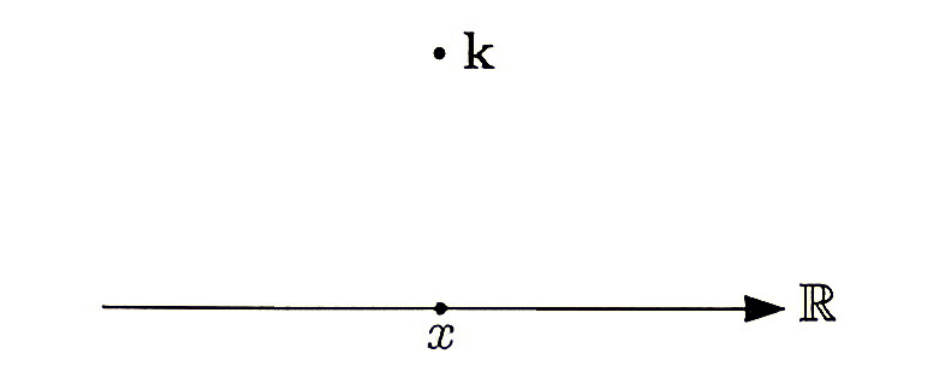
\includegraphics[width=0.5\linewidth]{figures/fig_p300_1.png}
  \caption*{图 10.2\quad $\R$ 上的摩天层（原书 p.292, Figure 10.2；PDF p.300）}
\end{figure}

% >>> p301
\begin{wexam}{10.2.7（结构层，structure sheaf）}
  设 $X$ 是光滑流形。\textbf{结构层} $\mathcal{O}_X$ 定义为
  \begin{equation}\tag{10.6}
    \mathcal{O}_X(U):=\{\text{光滑函数 } f\colon U\to\mathbf{k}\}
  \end{equation}
  （对任意 $U\in\operatorname{Op}(X)$）。若在 $\operatorname{Op}(X)$ 中 $U\subset V$，则限制映射
  $\operatorname{res}_{V,U}\colon\mathcal{O}_X(V)\to\mathcal{O}_X(U)$ 定义为函数
  从定义域 $V$ 到定义域 $U$ 的限制。此外，可以通过定义 $\mathcal{O}_X^\ast(U)$ 为
  $U$ 上所有处处非零的光滑函数之集，得到 $\mathcal{O}_X$ 的一个（子层）层。注意
  指数映射 $\exp\colon\mathcal{O}_X\to\mathcal{O}_X^\ast$ 是一个层态射。

  更具体地，取 $X=\C\setminus\{0\}$ 与 $\mathbf{k}=\C$。观察到
  $\operatorname{im}(\exp)$ 不是层，因为复对数只局部存在。这给出了练习 10.2.2 中
  所述「像层」问题的一个反例。

  最后注意：对任意拓扑空间 $X$，我们有下述层正合列
  \[
    0\to\Z_X\to\mathcal{O}_X\xrightarrow{\exp}\mathcal{O}_X^\ast\to0,
  \]
  其中 $\Z_X$ 表示阿贝尔群 $\Z$ 的（秩 1 的）常值层。
  \hfill$//$
\end{wexam}

下述练习提供了「烹调」更多层例子的方法。

\begin{wexer}{10.2.5}
  设 $X$ 是拓扑空间，$\mathcal{F}$ 是 $X$ 上的层。
  \begin{enumerate}[label=(\roman*)]
    \item 证明：对任意 $U\in\operatorname{Op}(X)$，定义在 $\operatorname{Op}(U)$ 上的限制
          $\mathcal{F}|_U$ 也是层（称为\textbf{限制层}）。
    \item 通过要求对每个 $x\in X$ 存在 $x$ 在 $X$ 中的邻域 $U$，使得限制层
          $\mathcal{F}|_U$ 是 $U$ 上的常值层，来定义 $X$ 上的层 $\mathcal{F}$。
          这样的层称为\textbf{局部常值层}（locally constant sheaf）。请给出一个
          是局部常值层但不是常值层的例子。
  \end{enumerate}
\end{wexer}

沿用与例 10.2.6 相同的精神——用茎来刻画层——下面是一个相当实用的问题。

\begin{wque}{10.2.1}
  给定拓扑空间 $X$ 上的层 $\mathcal{F}$，对局部闭子集 $Z\subset X$（即
  $Z=A\cap V$，其中 $A$ 在 $X$ 中闭、$V$ 在 $X$ 中开），如何烹调出 $X$ 上的一个
  层 $\mathcal{G}$，使得
  \[
    \mathcal{G}_x=\begin{cases}
      \mathcal{F}_x & \text{若 } x\in Z,\\
      0 & \text{否则}
    \end{cases}\quad?
  \]
\end{wque}

为实现这一点，需要对 $\mathcal{F}$ 施加一些运算。层论中有六种强大的层运算，通常称为
\textbf{Grothendieck 六种运算}（Grothendieck's six operations）。这些函子很重要，
特别是在以某种偏好的方式「裁剪」给定层时（例如问题 10.2.1）。下面我们介绍其中两种。

\begin{wdefn}{10.2.7（拉回，pullback）}
  给定拓扑空间 $X$、$Y$ 与 $Y$ 上的层 $\mathcal{F}$，设 $f\colon X\to Y$ 是连续
  映射。则 $\mathcal{F}$ 在 $f$ 下的\textbf{逆像（拉回）}（inverse image /
  pullback）定义为
% >>> p302
  \[
    (f^{-1}\mathcal{F})(U):=\varinjlim_{\substack{V\in\operatorname{Op}(Y)\\ f(U)\subset V}}
    \mathcal{F}(V),
  \]
  再加上必要的层化（见练习 10.2.1）。所得的层仍记作 $f^{-1}\mathcal{F}$。
\end{wdefn}

\begin{wexam}{10.2.8}
  (i) 设 $Y=\{\mathrm{pt}\}$ 是单点，则 $Y$ 上任何层 $\mathcal{F}$ 都是常值层。
  于是对常值映射 $f\colon X\to\{\mathrm{pt}\}$，由定义 10.2.7 有
  \[
    (f^{-1}\mathcal{F})(U)=\mathcal{F}(\{\mathrm{pt}\})
  \]
  对任意非空 $U\in\operatorname{Op}(X)$ 成立。这意味着 $f^{-1}\mathcal{F}$ 也是常值层。

  (ii) 给定拓扑空间 $X$、$Y$ 与 $Y$ 上的层 $\mathcal{F}$，对任意 $x\in X$，设
  $f\colon X\to Y$ 是 $X$ 到 $Y$ 的映射。则可以计算
  \begin{align*}
    (f^{-1}\mathcal{F})_x
    &=\varinjlim_{U\in\operatorname{Op}(X,x)}(f^{-1}\mathcal{F})(U)\\
    &=\varinjlim_{U\in\operatorname{Op}(X,x)}
    \varinjlim_{\substack{V\in\operatorname{Op}(Y)\\ f(U)\subset V}}\mathcal{F}(V)\\
    &=\varinjlim_{V\in\operatorname{Op}(Y,f(x))}\mathcal{F}(V)=\mathcal{F}_{f(x)}.
  \end{align*}
  因此，这说明 $f^{-1}$ 是\emph{正合函子}，其意义是：对 $Y$ 上任意层正合列
  $0\to\mathcal{F}\to\mathcal{G}\to\mathcal{H}\to0$，$X$ 上有正合列
  $0\to f^{-1}\mathcal{F}\to f^{-1}\mathcal{G}\to f^{-1}\mathcal{H}\to0$
  （见练习 10.2.4）。

  (iii) 设 $Z\subset Y$ 是拓扑空间 $Y$ 的子集，$j$ 是从 $Z$ 到 $Y$ 的包含映射。
  给定 $Y$ 上的层 $\mathcal{F}$，我们可以把层 $j^{-1}\mathcal{F}$（也记作
  $\mathcal{F}|_Z$）看作 $Z$ 上的层。容易验证：对任意 $x\in Z$，茎
  $(\mathcal{F}|_Z)_x$ 等于茎 $\mathcal{F}_x$。这几乎回答了上面的问题 10.2.1，
  只差一点：$\mathcal{F}|_Z$ 不是定义在 $Y$ 上（只定义在 $Z$ 上）。缺失的一步是
  从 $Z$ 到 $Y$ 的「延拓」。
  \hfill$//$
\end{wexam}

\begin{wdefn}{10.2.8（前推，pushforward）}
  设 $\mathcal{F}$ 是 $X$ 上的层，则对任意连续映射 $f\colon X\to Y$，层
  $\mathcal{F}$ 在 $f$ 下的\textbf{直接像（前推）}（direct image / pushforward）
  由
  \[
    (f_\ast\mathcal{F})(V):=\mathcal{F}\bigl(f^{-1}(V)\bigr)
  \]
  对任意 $V\in\operatorname{Op}(Y)$ 定义。这已经是层。
\end{wdefn}

让我们在与例 10.2.8 相同的框架下做一些计算。

\begin{wexam}{10.2.9}
  (i) 考虑 $f\colon X\to Y$，其中 $Y=\{\mathrm{pt}\}$ 是单点。则对 $X$ 上的层
  $\mathcal{F}$，它在 $f$ 下的前推是 $\{\mathrm{pt}\}$ 上的层，显然是一个常值层。
  为描述这个常值层，由定义 10.2.8 有
  \[
    (f_\ast\mathcal{F})(Y)=\mathcal{F}\bigl(f^{-1}(Y)\bigr)=\mathcal{F}(X),
  \]

% >>> p303
  它由整个空间 $X$ 上的所有截面组成。任何这样的截面 $s\in\mathcal{F}(X)$ 称为
$\mathcal{F}$ 的\textbf{整体截面}（global section）。就记号而言，$\mathcal{F}(X)$
常记作 $\Gamma(X,\mathcal{F})$。之所以要提及并引入这个新记号，是因为后文取层的整体
截面（记作 $\Gamma(X,\cdot)$）也将是一个经常出现的运算。

(ii) 与例 10.2.8 (ii) 类似，可以计算前推的茎：
\[
  (f_\ast\mathcal{F})_y
  =\varinjlim_{V\in\operatorname{Op}(Y,y)}(f_\ast\mathcal{F})(V)
  =\varinjlim_{V\in\operatorname{Op}(Y,y)}\mathcal{F}\bigl(f^{-1}(V)\bigr).
\]
要注意：即使 $x\in f^{-1}(y)$，计算结果 $(f_\ast\mathcal{F})_y$ 也可能与
$\mathcal{F}_x$ 不同。例如，取 $X=\{a,b\}$ 配以离散拓扑（即
$\operatorname{Op}(X)=\{\varnothing,\{a\},\{b\},\{a,b\}\}$），$Y=\{a\}$，考虑常值映射
$f\colon X\to Y$。取定义 10.2.6 中 $X$ 上的摩天层 $\underline{a}$。则
\[
  (f_\ast\underline{a})_a
  =(f_\ast\underline{a})(\{a\})
  =\underline{a}\bigl(f^{-1}(\{a\})\bigr)
  =\underline{a}(\{a,b\})=\mathbf{k},
\]
而当 $b\in f^{-1}(\{a\})$ 时茎 $\underline{a}_b=0$。

(iii) 设 $Z\xrightarrow{j}Y$ 是拓扑空间 $Z$ 到拓扑空间 $Y$ 的包含映射。则由
定义 10.2.8，对 $Z$ 上的层 $\mathcal{F}$ 有
\[
  (j_\ast\mathcal{F})(U)=\mathcal{F}(U\cap Z)
\]
  对任意 $U\in\operatorname{Op}(Y)$ 成立。注意 $U\cap Z$ 在 $Y$ 中未必是开集，但由子空间拓扑，
  它是 $\operatorname{Op}(Z)$ 中的元素。
  \hfill$//$
\end{wexam}

若把例 10.2.8 (iii) 与例 10.2.9 (iii) 结合起来，在 $Z\xrightarrow{j}Y$ 的框架下
给定 $Y$ 上的层 $\mathcal{F}$，则可以用下述方式「裁剪」$\mathcal{F}$：
\begin{equation}\tag{10.7}
  \mathcal{F}
  \xrightarrow{\ \text{限制}\ }
  j^{-1}\mathcal{F}
  \xrightarrow{\ \text{延拓}\ }
  j_\ast\bigl(j^{-1}\mathcal{F}\bigr).
\end{equation}

\begin{wexam}{10.2.10}
  考虑 $Z:=[0,1]\xrightarrow{j}\R=:Y$。给定常值层
  $\mathcal{F}=\mathbf{k}_Y$，其中对任意非空 $U\in\operatorname{Op}(Y)$ 有
  $\mathbf{k}_Y(U)=\mathbf{k}$。我们可以考察一些茎。例如
  \begin{align*}
    \bigl(j_\ast(j^{-1}\mathbf{k}_Y)\bigr)_0
    &=\varinjlim_{U\in\operatorname{Op}(\R,0)}j^{-1}\mathbf{k}_Y\bigl(j^{-1}(U)\bigr)\\
    &=\varinjlim_{\varepsilon\to0}\bigl(j^{-1}\mathbf{k}_Y\bigr)([0,\varepsilon))\\
    &=\varinjlim_{\varepsilon\to0}
    \varinjlim_{V\supset[0,\varepsilon)}\mathbf{k}_Y(V)\\
    &=\varinjlim_{\varepsilon\to0}\mathbf{k}_Y\bigl((-\varepsilon,\varepsilon)\bigr)
    =\mathbf{k}.
  \end{align*}
  类似地，可以算出 $\bigl(j_\ast(j^{-1}\mathbf{k}_Y)\bigr)_1=\mathbf{k}$。
  \hfill$//$
\end{wexam}

一般地，对\emph{闭}子集 $Z\subset Y$，我们有下述命题。

% >>> p304
\begin{wprop}{10.2.1}
  设 $Z\subset Y$ 是闭子空间。则对 $Y$ 上的任意层 $\mathcal{F}$，层
  $j_\ast(j^{-1}\mathcal{F})$ 的茎满足
  \[
    \bigl(j_\ast(j^{-1}\mathcal{F})\bigr)_x=\mathcal{F}_x
    \qquad\text{对任意 } x\in Z,
  \]
  而对任意 $x\notin Z$ 它为零。
\end{wprop}

这就在 $Z$ 是（$Y$ 的）闭子空间时回答了问题 10.2.1。然而，当把 $Z$ 换成开子空间时，
例如取 $Z:=(0,1)\subset\R=:Y$，与例 10.2.10 相同的计算表明
\[
  \bigl(j_\ast(j^{-1}\mathbf{k}_Y)\bigr)_0
  =\bigl(j_\ast(j^{-1}\mathbf{k}_Y)\bigr)_1=\mathbf{k},
\]
而这\emph{不是}问题 10.2.1 所要求的。为解决这一问题，下面给出处理 $Y$ 中开子空间的一个
巧妙办法。仍在具体框架 $Z=(0,1)\subset\R=Y$ 中，考虑补集 $\R\setminus(0,1)$，它是
$Y$ 的闭子空间。于是对包含映射 $i\colon\R\setminus(0,1)\to\R$，由命题 10.2.1，我们
可以把 $\mathbf{k}_Y$ 裁剪为 $i_\ast(i^{-1}(\mathbf{k}_Y))$。关键观察是：存在一个
由限制诱导的层态射
$\mathbf{k}_Y\to i_\ast(i^{-1}\mathbf{k}_Y)$。事实上，更一般地，对任意子空间包含
$Z\xrightarrow{j}Y$ 与 $Y$ 上的层 $\mathcal{F}$，存在由限制诱导的层态射
\begin{equation}\tag{10.8}
  \mathcal{F}\to j_\ast\bigl(j^{-1}\mathcal{F}\bigr).
\end{equation}
具体地说，对任意 $U\in\operatorname{Op}(Y)$，有
\begin{equation}\tag{10.9}
  \mathcal{F}(U)\to j_\ast(j^{-1}\mathcal{F})(U)
  =(j^{-1}\mathcal{F})(U\cap Z)
  =\varinjlim_{U\cap Z\subset V}\mathcal{F}(V).
\end{equation}
于是，依照 (10.9)，可以计算下述核层在 $0$ 处的茎：
\begin{align*}
  \ker\bigl(\mathbf{k}_X\to i_\ast(i^{-1}\mathbf{k}_X)\bigr)_0
  &=\varinjlim_{U\in\operatorname{Op}(\R,0)}
  \ker\bigl(\mathbf{k}_X(U)\to i_\ast(i^{-1}\mathbf{k}_X)(U)\bigr)\\
  &=\varinjlim_{\varepsilon\to0}
  \ker\bigl(\mathbf{k}_X((-\varepsilon,\varepsilon))
  \to i_\ast(i^{-1}\mathbf{k}_X)((-\varepsilon,\varepsilon))\bigr)\\
  &=\varinjlim_{\varepsilon\to0}\ker\bigl(\mathbf{k}
  \xrightarrow{\mathbf{1}_{\mathbf{k}}}\mathbf{k}\bigr)=0.
\end{align*}

% [Tutor Note: 原文疑误（记号不一致）——本段的框架是 $Z=(0,1)\subset\R=Y$、
% $i\colon\R\setminus(0,1)\to\R$，故所裁剪的常值层应是 $\mathbf{k}_Y$（环境空间
% $Y=\R$ 上的常值层）；但原书此处印作 $\mathbf{k}_X$（以及 $i_\ast(i^{-1}\mathbf{k}_X)$）。
% 这很可能是 $Y$ 误写成 $X$。译文保留原文的 $\mathbf{k}_X$ 写法，已记入
% review_ch10a.md，建议核对原书。]

一般地，关于开子空间我们有下述命题。

\begin{wprop}{10.2.2}
  设 $Z\subset Y$ 是开子空间，$i\colon Y\setminus Z\to Y$ 是补集的包含映射，则核层
  $\ker\bigl(\mathcal{F}\to i_\ast(i^{-1}\mathcal{F})\bigr)$ 满足命题 10.2.1 中
  的茎性质。
\end{wprop}

因此，这就在 $Z$ 是（$Y$ 的）开子空间时回答了问题 10.2.1。更一般地，考虑局部闭子集
$Z=A\cap V\subset Y$，其中 $A$ 是开子空间、$V$ 是 $Y$ 中的闭子空间，我们可以定义层
\begin{equation}\tag{10.10}
  \mathcal{F}_Z:=(\mathcal{F}_V)_A.
\end{equation}

% >>> p305
这里，$\mathcal{F}_V$ 定义为 $j_\ast(j^{-1}\mathcal{F})$，其中 $j$ 是从 $V$ 到
$Y$ 的包含映射；而 $(\mathcal{F}_V)_A$ 定义为
$\ker\bigl(\mathcal{F}_V\to i_\ast(i^{-1}\mathcal{F}_V)\bigr)$，其中 $i$ 是从
$X\setminus A$ 到 $Y$ 的包含映射。于是可以验证 $\mathcal{F}_Z$ 的茎满足问题 10.2.1
所要求的性质：
\[
  (\mathcal{F}_Z)_y=\begin{cases}
    \mathcal{F}_y & \text{若 } y\in Z,\\
    \varnothing & \text{否则}
  \end{cases}
\]
这样的运算 $\mathcal{F}\mapsto\mathcal{F}_Z$ 可以粗略地表述为「裁剪 $\mathcal{F}$
（但仍定义在 $Y$ 上），只保留 $Z\subset Y$ 的信息」。

此外，由于 (10.8)，存在层态射 $\mathcal{F}\to\mathcal{F}_Z$。固定任意局部闭子集
$Z\subset Y$，对应 $\mathcal{F}\to\mathcal{F}_Z$ 满足下述性质（见 [135] 中命题
2.3.6）：
\begin{enumerate}[label=(\roman*)]
  \item 对应 $\mathcal{F}\mapsto\mathcal{F}_Z$ 是正合的（见例 10.2.8 (ii)）。
  \item 给定另一个局部闭子集 $Z'$，对应
        $\mathcal{F}_Z\mapsto(\mathcal{F}_Z)_{Z'}$（按与 (10.10) 相同的方式定义）
        等于 $\mathcal{F}_{Z\cap Z'}$。
  \item 若 $Z'\subset Z(\subset X)$ 在 $Z$ 中闭，则 $X$ 上有层正合列
        \begin{equation}\tag{10.11}
          0\to\mathcal{F}_{Z\setminus Z'}\to\mathcal{F}_Z\to\mathcal{F}_{Z'}\to0.
        \end{equation}
        这里，$\mathcal{F}_Z\to\mathcal{F}_{Z'}$ 由限制诱导，而
        $\mathcal{F}_{Z\setminus Z'}$ 是态射 $\mathcal{F}_Z\to\mathcal{F}_{Z'}$
        的核层。
\end{enumerate}

\begin{wrem}{10.2.4}
  上面性质 (ii) 蕴含：在 (10.10) 中，可以交换关于 $V$ 与 $A$ 的裁剪次序。
\end{wrem}

上面性质 (iii) 是一个方便的性质，使我们能够考察更多层的例子。下述例子很受欢迎。

\begin{wexam}{10.2.11}
  考虑 $Z=(0,1]\subset\R$，并令 $\mathcal{F}$ 为 $\R$ 上秩 1 的常值层
  $\mathbf{k}_\R$。则可以利用由 (10.11) 得到的下述正合列来研究
  $(\mathbf{k}_\R)_{(0,1]}$。由于 $(-\infty,0]$ 在 $(-\infty,1]$ 中闭，我们有下述
  短正合列
  \begin{equation}\tag{10.12}
    0\to(\mathbf{k}_\R)_{(0,1]}\to(\mathbf{k}_\R)_{(-\infty,1]}
    \to(\mathbf{k}_\R)_{(-\infty,0]}\to0.
  \end{equation}
  集中在 $x=0$ 处，上述正合列转化为
  \[
    0\to\bigl((\mathbf{k}_\R)_{(0,1]}\bigr)_0
    \to\bigl((\mathbf{k}_\R)_{(-\infty,1]}\bigr)_0
    \to\bigl((\mathbf{k}_\R)_{(-\infty,0]}\bigr)_0\to0,
  \]
  这蕴含 $\bigl((\mathbf{k}_\R)_{(0,1]}\bigr)_0=0$。更一般地，通过简单计算（练习），
  我们知道对任意开子集 $(a,b)\in\operatorname{Op}(\R)$，
  \[
    \bigl((\mathbf{k}_\R)_{(-\infty,1]}\bigr)\bigl((a,b)\bigr)
    =\begin{cases}
      \mathbf{k} & \text{若 } a<1,\\
      0 & \text{若 } a\ge1.
    \end{cases}
  \]

% [Tutor Note: 原文疑误（待核对）——上述截面公式只以左端点 $a$ 为条件，但按裁剪层的
% 定义 (10.10)，对跨越边界的区间（如 $a<1<b$）截面应为 $a<1$ 时的常值 $\mathbf{k}$
% 这一段「落在 $(-\infty,1]$ 内」的部分；而对 $a\ge1$ 为零。对
% $(\mathbf{k}_\R)_{(-\infty,1]}$ 而言这与印刷公式一致（因为补集 $[2,\infty)$ 与
% $U\cap(-\infty,1]$ 不相交），故 (10.12) 后的公式正确；但下一节的端点约定
% （$a=1$ 处闭开）可能需与原书核对。]

% >>> p306
类似地，
\[
  \bigl((\mathbf{k}_\R)_{(-\infty,0]}\bigr)\bigl((a,b)\bigr)
  =\begin{cases}
    \mathbf{k} & \text{若 } a<0,\\
    0 & \text{若 } a\ge0.
  \end{cases}
\]
于是，由于 $(\mathbf{k}_\R)_{(0,1]}$ 可以等同于
$(\mathbf{k}_\R)_{(-\infty,1]}\to(\mathbf{k}_\R)_{(-\infty,0]}$ 的核层，我们有
\begin{align*}
  \bigl((\mathbf{k}_\R)_{(0,1]}\bigr)\bigl((a,b)\bigr)
  &=\ker\Bigl(\bigl((\mathbf{k}_\R)_{(-\infty,1]}\bigr)\bigl((a,b)\bigr)
  \to\bigl((\mathbf{k}_\R)_{(-\infty,0]}\bigr)\bigl((a,b)\bigr)\Bigr)\\
  &=\begin{cases}
    \mathbf{k} & \text{若 } a\in[0,1],\\
    0 & \text{否则},
  \end{cases}
\end{align*}
  这就对开区间算出了 $(\mathbf{k}_\R)_{(0,1]}$。
  \hfill$//$
\end{wexam}

% [Tutor Note: 原文疑误（端点约定）——按上式，对 $a=1$ 有
% $(\mathbf{k}_\R)_{(-\infty,1]}((a,b))=\mathbf{k}$ 而
% $(\mathbf{k}_\R)_{(-\infty,0]}((a,b))=0$，故核为 $\mathbf{k}$；但若 $b\le1$ 且
% $a=1$ 则区间为空。原书写「$a\in[0,1]$」，端点 $a=1$ 处的开闭约定与原书所用的
% 「左开右闭」区间约定可能不一致。已记入 review_ch10a.md 待核对。]

\par\medskip\noindent\textbf{记号}\quad 我们引入下述记号：$\operatorname{Sh}(\mathbf{k}_X)$ 表示拓扑空间 $X$ 上
（$\mathbf{k}$-模）层构成的范畴。则 $f_\ast$、$f^{-1}$ 与 $\cdot_Z$（对局部闭子集
$Z\subset X$）是 $\operatorname{Sh}(\mathbf{k}_X)$ 上的三个函子，其中由上述讨论，
$f^{-1}$ 与 $\cdot_Z$ 都是正合函子。记
$\mathbf{k}_Z:=(\mathbf{k}_X)_Z$，其中 $\mathbf{k}_X$ 是 $X$ 上的常值层。特别地，
$\mathbf{k}_Z$ 定义在环境空间 $X$ 上。

为结束本节，我们陈述一个结构性的结果，它基于例 10.2.3 (iii) 中提到的
$\gamma$-拓扑。回忆：拓扑空间 $X$ 上的\textbf{可构造层}（constructible sheaf）是
这样的层——存在 $X$ 的有限多个局部闭子集，记作 $\{U_i\}_{i=1}^m$，满足
$X=\bigcup_{i=1}^m U_i$，且在每个 $U_i$ 上该层是局部常值的（见练习 10.2.5）。于是，
对 $\R_\gamma$ 上（即配以 $\gamma$-拓扑的 $\R$ 上）的可构造层，我们有下述结果。
这个结果可以看作持续 $\mathbf{k}$-模的分解结果——5.2 节中的定理 5.2.1——的层类比
（cf.\ 例 10.2.4 的 (iii)）。

\begin{wthm}{10.2.1（[104] 中的推论 7.3）}
  对 $\R_\gamma$ 上的任意可构造层 $\mathcal{F}$，它可以按下述方式分解为层的直和：
  \[
    \mathcal{F}\simeq\bigoplus_{I}\mathbf{k}_I,
  \]
  其中每个 $I$（可以出现多次）是 $\R$ 中形如 $(s,t]$ 的区间（$t$ 可以是 $\infty$）。
  此外，这样的分解在重新排列区间 $I$ 的意义下是唯一的。
\end{wthm}

定理 10.2.1 中分解的一幅示意图见图 10.3。

把定理 10.2.1 与 5.2 节中的定理 5.2.1 相比较，两者的「积木」都记作
$\mathbf{k}_I$。然而，按例 5.2.3，定理 5.2.1 中的 $\mathbf{k}_I$ 表示区间型持续
$\mathbf{k}$-模；而定理 10.2.1 中的 $\mathbf{k}_I$ 表示关于局部闭子集
$I\subset\R$ 裁剪的常值层（秩 1）。事实上，

% [Tutor Note: 术语/记号依据——「可构造层」在 $\R_\gamma$ 上的分解
% $\mathcal{F}\simeq\bigoplus_I\mathbf{k}_I$ 与持续模的条形码分解是同一个定理的两种
% 语言：区间 $(s,t]$ 对应条形码中的一条「条」，$\mathbf{k}_I$ 是全序集上的区间常值层，
% 其茎在 $I$ 内非零、在 $I$ 外为零。注意定理 10.2.1 中的 $\mathbf{k}_I$ 与定理 5.2.1
% 中的 $\mathbf{k}_I$ 同名而所指不同（前者是层，后者是持续模），这是原书有意为之的
% 记号统一，阅读时勿混淆。]

% （本页末句「It is in fact」未完，续见 PDF p307，由另一位译者接续。）
